\begin{abstract}
Can intermediate supervision teach a recurring transition quickly when final-answer supervision supplies exponentially weak credit? We establish a matched separation for modular counting in a concrete two-block causal softmax-attention/ReLU Transformer. Two population gradient flows start from the same aligned, small, structured initialization and train the same readouts and tied query--key scalars. Process supervision develops persistent positive margins on every recurring supervised transition in $O(n^{5/2}\log n)$ time at linear executor width; outcome supervision remains near initialization, with expected correct-answer probability near $1/K$, for $\Omega(\lambda^{-n})$ time. The positive result fixes the value features and supplies routing; the outcome plateau also holds for a broader joint-training family. Separate explicit constructions realize both complete programs in the overall architecture, without asserting their reachability in the restricted trained subspace. Counting measurements and pretrained Qwen2.5-0.5B LoRA experiments support the qualitative mechanism; a five-object BIG-Bench Hard reversal limits its empirical scope.
\end{abstract}

\section{Introduction}
A final answer can conceal many repeated state updates. A running trace exposes those updates as local prediction problems. The question is whether this changes optimization time within the same Transformer, rather than merely changing what the architecture can represent. We study counting modulo $K$: each independent letter either keeps the state or advances it by one. The answer space stays fixed as the computation grows.

Our principal result fixes one architecture, one initialization, one trainable parameter set, and population gradient flow. Only the objective and its associated teacher-forced continuation change. In an aligned supplied-routing regime,
\begin{equation}\label{eq:headline}
\boxed{T_{\mathrm{step}}=O(n^{5/2}\log n),\qquad T_{\mathrm{out}}=\Omega(\lambda^{-n}).}
\end{equation}
Here $T_{\mathrm{step}}$ is an upper bound on the time after which all recurring transition predictions have persistent positive margins. $T_{\mathrm{out}}$ is a lower bound on the duration of an initial plateau, measured by displacement, cross-entropy, and expected probability assigned to the correct answer. It is not a lower bound for reaching arbitrary accuracy, and it says nothing about permanent failure.

The mechanism has three stages. First, a feature that reads $k$ of $n$ independent letters sees answer-dependent correlation attenuated by $\lambda^{n-k}$. Second, a score expansion of the actual Transformer decomposes its local logits into terms with controlled letter support and scale. The resulting local loss floor bounds gradient-flow displacement over an exponential time interval. Third, the step objective directly exposes the state--letter transition. Exact parameter dynamics show how an asymmetric state prior bootstraps the trainable interaction, after which all competitor logits lose to the correct count.

The constructive result and the learning result address different questions. Explicit finite-score two-block executors realize direct final counts and full running traces at linear width. The positive learning proof uses a smaller family with fixed value maps, a supplied two-site mask, a full count readout, a restricted gate readout, and tied query--key scalars. Executor existence in the larger parameter space does not establish that the final-count executor lies in this training family. This distinction is essential to interpreting the separation.

The evidence also has distinct roles. Small-initialization counting runs measure displacement times and their dependence on horizon. Other counting runs measure actual rule learning outside the theorem's structured seed. Pretrained Qwen LoRA experiments test qualitative transfer to Boolean circuits and object tracking, including a case where outcome supervision performs better. None of those pretrained-model results proves the exponential bound.

\section{Modular counting and Transformer setup}\label{sec:setup}\label{sec:setting}
\begin{definition}[Task and contraction]\label{def:task}\label{def:lambda}
Fix $K\ge2$, a finite alphabet $\Sigma$, and a query letter $w^\star$ with probability $p\in(0,1)$. Independently sample $s_0$ uniformly from $\mathbb Z_K$ and letters $w_1,\ldots,w_n$. Put $b_t=\mathbf1[w_t=w^\star]$ and
\begin{equation}
s_t=s_{t-1}+b_t\pmod K,\qquad y=s_n,\qquad
\lambda=\max_{1\le j<K}|1-p+p e^{2\pi\mathrm i j/K}|.
\label{eq:lambda}
\end{equation}
For $p\ne1/2$, $0<\lambda<1$. In the binary case $\lambda=|1-2p|$.
\end{definition}
The prompt displays $s_0$, the query, and all letters. Outcome format predicts only the final count. Process format appends the running states, using gold previous states during training. At the position $i_t=n+1+t$ predicting $s_t$, $t\ge2$, the displayed token is $s_{t-1}$; the current letter is at $j_t=1+t$. The first state prediction is a separate boundary case.

\begin{definition}[Population objectives]\label{def:losses}
With $z_t(\vartheta)\in\mathbb R^K$ the count logits predicting $s_t$ and $z_{\mathrm{ans}}(\vartheta)$ the outcome-answer logits, define
\begin{equation}\label{eq:objectives}
\Lout=\E[-\log\softmax(z_{\mathrm{ans}})_y],\qquad
\Lstep=\frac1{n-1}\sum_{t=2}^n\E[-\log\softmax(z_t)_{s_t}].
\end{equation}
The theorem covers this recurring-transition loss, not the boundary prediction or a complete autoregressive rollout from an unpredicted first state.
\end{definition}

\paragraph{Overall architecture.}\label{ass:arch}
Each of two residual blocks has three causal softmax-attention heads and a ReLU MLP. There is no LayerNorm. A head may use a fixed input-independent causal submask. With $h_i^0=E(\mathrm{token}_i)+P_i$, each block computes
\begin{align}
\bar h_i^\ell&=h_i^{\ell-1}+\sum_{a=1}^3\sum_{j\in\mathcal M_a(i)}\omega_{ij}^{\ell,a} W_V^{\ell,a}h_j^{\ell-1},\nonumber\\
\omega_{ij}^{\ell,a}&=\softmax_{j\in\mathcal M_a(i)}\left(\frac{(W_Q^{\ell,a}h_i^{\ell-1})^\top W_K^{\ell,a}h_j^{\ell-1}}{\sqrt{d_{\mathrm h}}}+\beta_{i-j}^{\ell,a}\right),\label{eq:block}\\
h_i^\ell&=\bar h_i^\ell+W_{\mathrm{out}}^\ell\relu(W_{\mathrm{in}}^\ell\bar h_i^\ell+b^\ell),\qquad z_i=Vh_i^2.\nonumber
\end{align}
The value map includes the map back to the residual stream. The executor construction in \cref{app:architectures} specifies every register and nonzero tensor. At fixed $K,|\Sigma|$, head dimension, residual width, and MLP width are $\Theta(n)$.

\paragraph{The structured seed and trained family.}\label{sec:seed}
Let $R e_s=e_{s+1}$, and fix orthonormal residual directions $\hat e_0,\hat e_\ell$, count and gate registers $(\hat e_s^{\mathrm c})_s,(\hat e_s^{\mathrm g})_s$, and a unit head vector $\hat e_{\mathrm h}$. The nonzero token embeddings are
\[
E(s)=\varepsilon\hat e_s^{\mathrm c},\quad
E(w^\star)=\varepsilon(\hat e_0-\hat e_\ell),\quad
E(w\ne w^\star)=\varepsilon(\hat e_0+\hat e_\ell).
\]
Position and format-token embeddings are zero. Only head 1 of block 2 is active. Its mask at $i_t$ admits $i_t,j_t$, and its maps are
\begin{equation}\label{eq:seedmaps}
W_Q=q\Pi_Q,\quad W_K=k\Pi_K,\quad W_V=v\Pi_V,
\end{equation}
where $\Pi_Q=\sum_s\hat e_{\mathrm h}(\hat e_s^{\mathrm c})^\top$, $\Pi_K=\hat e_{\mathrm h}\hat e_\ell^\top$, and $\Pi_V=\sum_s\hat e_s^{\mathrm g}(\hat e_s^{\mathrm c})^\top$. All other heads and MLP weights vanish; every MLP bias is $\pm\varepsilon$. Relative biases are zero and fixed. At outcome-answer positions choose any fixed nonempty causal visible set, independent of the input, and use that same mask in both models.

The readout blocks are $U$ on the count register and $W=w(I-R)$ on the gate register. Train
\begin{equation}\label{eq:metric}
\vartheta=(U,W,q,k)\in\mathbb R^{K\times K}\times\mathbb R(I-R)\times\mathbb R^2,
\quad \|\vartheta\|^2=\|U\|_F^2+\|W\|_F^2+q^2+k^2.
\end{equation}
Both objectives use this metric: $\dot\vartheta=-\nabla_\vartheta\mathcal L$. All embeddings, value maps, MLPs, other heads, masks and biases remain fixed. The initialization is
\begin{equation}\label{eq:init}
U_0=W_0=0,\quad \varepsilon/2\le|q_0|,|k_0|,|v|\le2\varepsilon,
\quad q_0k_0(1-2p)<0.
\end{equation}
The architecture has two blocks, although this restricted seed activates only one head. The positive theorem does not prove discovery of the mask or feature roles.

\section{Exact executors and the matched theorem}\label{sec:results}
\begin{proposition}[Exact Outcome and Step Executors Exist in the Same Two-Block Transformer]\label{prop:represent}
For every $n\ge2$, $K\ge2$ and finite $\Sigma$, the architecture of \cref{eq:block} with full causal masks, three heads per block, $d_{\mathrm h}=2n+6$, $d_{\mathrm{res}}=2|\Sigma|+4K+d_{\mathrm h}+3$, and MLP width $\max\{|\Sigma|,3K(n+1),2n+1\}$ admits separate parameter settings that greedily generate the entire running-count continuation and the direct final-count continuation on every prompt. Every required prediction has strictly positive logit margin.
\end{proposition}
\begin{proof}[Construction idea]
Block 1 retrieves the query and computes its match with each letter by a ReLU equality test. The step executor retrieves the previous state and the next match bit and applies a modular lookup. The outcome executor averages match bits, rescales to the count, retrieves $s_0$, and applies a triangular-ReLU lookup. Finite softmax scores make retrieval approximate, but the explicit leakage bound preserves the logit margins. The complete construction and finite-score proof are in \cref{app:architectures}; exhaustive verification is separate in \cref{app:verify}.
\end{proof}
This proposition concerns the overall architecture. Its parameters differ substantially from the small structured seed, and its outcome executor need not be reachable with only \cref{eq:metric} trainable.

\begin{theorem}[Exponential Separation Between Outcome and Process Supervision in a Two-Block Transformer]\label{thm:matched}\label{thm:outcome-end}
Fix $K\ge2$, $p\in(0,1)\setminus\{1/2\}$ and $n\ge2$. Use \cref{def:task,eq:block,sec:seed}, the common seed \cref{eq:init}, and the common metric and trainable family \cref{eq:metric}. Let $h^\star=|\log((1-p)/p)|$, $p_{\min}=\min(p,1-p)$, and $r_0=1/8$. Let $N_b$ bound the scaled MLP-bias vector norms. There exist $c_{\mathrm{init}},c_\lambda,C_2>0$, depending only on fixed $K$ and the block/head counts and scaled operator-norm bounds, such that the following holds whenever
\begin{equation}\label{eq:small}
0<\varepsilon\le\min\{1/2,c_{\mathrm{init}}\min(1,N_b^{-1}),c_\lambda\lambda\}.
\end{equation}
Run two independent population gradient flows for \cref{eq:objectives} from this seed. Write $\theta$ for their embedding in the overall Transformer parameter space.
\begin{enumerate}[label=(\roman*),leftmargin=*,itemsep=2pt]
\item For $0\le t\le T_{\mathrm{out}}:=r_0^2\lambda^{-n}/(2KC_2)$, the outcome flow satisfies
\begin{align}
\|\theta_{\mathrm{out}}(t)-\theta_0\|&\le r_0\varepsilon,\nonumber\\
\log K-C_2\varepsilon^2\lambda^n\le\Lout(t)&\le\log K,\label{eq:plateau}\\
\left|\E[\softmax(z_{\mathrm{ans}}(t))_y]-1/K\right|&\le\sqrt{C_2/2}\,\varepsilon\lambda^{n/2}.\nonumber
\end{align}
The displacement uses the ambient Frobenius norm, including all fixed blocks.
\item There is a time $t_3\le T_{\mathrm{step}}$ after which every supervised recurring transition has positive margin against all $K-1$ wrong counts, persistently for all $t\ge t_3$, and $\Lstep(t)\to0$. An explicit upper bound is
\begin{equation}\label{eq:focused-time}
\begin{split}
T_{\mathrm{step}}={}&\frac{h^\star}{4\rho\varepsilon^2\mu}
+\frac{4080\sqrt{d_{\mathrm h}}}{p_{\min}\min\{1,h^\star\}\varepsilon^4}
\log\frac{8\sqrt{d_{\mathrm h}}}{\varepsilon^4}
+\frac{8010K\log K}{p_{\min}^2\varepsilon^4},\\
&\rho=2/K,\qquad \mu=p_{\min}(1-2p_{\min})/14.
\end{split}
\end{equation}
\item If $T_{\mathrm{step}}<T_{\mathrm{out}}$, both conclusions hold on $[T_{\mathrm{step}},T_{\mathrm{out}}]$. At fixed $K,p$, executor widths $d_{\mathrm h},w=\Theta(n)$ and $\varepsilon=c_*n^{-1/2}$ with a sufficiently small fixed $c_*>0$, this overlap holds for all sufficiently large $n$, and \cref{eq:headline} follows.
\end{enumerate}
\end{theorem}
The constants $c_{\mathrm{init}},c_\lambda,C_2$ are the local-bound constants in \cref{ass:init,lem:score-sum,lem:bias-uniform}, not measured numerical values. The factor $K$ in the plateau duration accounts for the tied scalar metric, as proved in \cref{app:match}. The principal theorem is restricted to aligned seeds; it does not need a query--key magnitude-gap condition.

\paragraph{What the observables mean.}
Positive transition margins imply correct greedy transition predictions given the gold previous state. The outcome probability bound controls the average probability assigned to the correct answer; it does not bound greedy accuracy, which can be sensitive to arbitrarily small logit differences. Cross-entropy and displacement have separate bounds. The theorem's two flows share parameters at time zero and trainable directions, not trajectories or teacher-forced inputs.

\section{Why learning times separate}\label{sec:credit}
\paragraph{A. Unseen letters contract outcome credit.}
Let $\xi=e_y-\mathbf1/K$. Fix the query and $s_0$. For $S\subseteq[n]$, Fourier conditioning gives
\begin{equation}\label{eq:credit-degree}
\|\E[H^\top\xi]\|\le\lambda^{n-|S|}\|H\|_{L^2}
\end{equation}
for every square-integrable matrix $H$ measurable in $w_S$. Each omitted Bernoulli increment multiplies the $j$th Fourier mode by $1-p+p e^{2\pi\mathrm i j/K}$. \Cref{lem:target-contraction} proves the exact conditional norm identity.

Inside a fixed-ReLU neighborhood, scale every content attention score by $\zeta$ and Taylor expand at $\zeta=0$. A term of score order $k$ reads at most $2k+1$ letters. Its Jacobian has absolute-sum bound $C\varepsilon^2(C_{\mathrm{att}}\varepsilon^4)^k$ for $k\ge1$. The zero-order network is affine in individual inputs. These are estimates for \cref{eq:block}; they follow from the softmax derivative recursion and two-block composition, not from replacing the Transformer by a low-degree predictor. Summing \cref{eq:credit-degree} with a bounded Taylor remainder yields
\[
|\E\langle z,\xi\rangle|\le C_2\varepsilon^2\lambda^n.
\]
The complete parameter-scale, support and remainder arguments are in \cref{app:outcome}.

\paragraph{B. The local loss floor limits displacement.}
Write $u=\mathbf1/K$, $p_\theta=\softmax(z)$ and $C_{\mathrm{out}}=\E\langle z,e_y-u\rangle$. The exact identity
\[
\Lout=\log K+\E\KL(u\|p_\theta)-C_{\mathrm{out}}
\]
turns weak credit into a local loss floor. At the zero readout the loss is $\log K$. Along gradient flow in its training metric,
$\int_0^t\|\dot\vartheta\|^2=\Lout(0)-\Lout(t)$.
Cauchy--Schwarz then bounds displacement by the square root of time times the possible loss decrease. Pinsker's inequality bounds expected correct-answer probability separately. Norm comparison transfers this argument to the tied scalar family in \cref{app:match}. The local outcome proof also permits broader full joint flow and trained relative biases; that freedom is not part of the positive theorem.

\paragraph{C. The displayed state bootstraps a rule.}
The active Transformer head gives exactly
\begin{equation}\label{eq:actual-features}
z_t=\varepsilon Ue_{s_{t-1}}+\varepsilon v r_{b_t}We_{s_{t-1}},\qquad
r_b=\sigma(-(-1)^b a),\quad a=\varepsilon^2qk/\sqrt{d_{\mathrm h}}.
\end{equation}
Cyclic data symmetry preserves a circulant count readout, and permutation symmetry makes the background offsets equal. The induced coordinates are the count contrast $c$, gate contrast $g=2\varepsilon vw$, and background height $s$ in \cref{lem:J-reduce}. Their useful margins and rule contrast are
\begin{equation}\label{eq:rule}
m_b=(-1)^b(c+gr_b),\qquad R=m_0+m_1=-g\tanh(a/2).
\end{equation}
The count-only component cancels in $R$. This contrast is necessary for learning both transitions, but positivity of $R$ alone is insufficient. The proof tracks the loss and all background logits as well.

For $p<1/2$ the state prior favors staying, so it first moves the count readout. Alignment $a(0)<0$ makes the same signal increase the gate readout in the useful direction. A balance identity preserves alignment and yields a persistent floor $g\gtrsim\varepsilon^2\min(1,h^\star)$. Before the loss crosses its success threshold, $|a|$ grows at a rate at least a constant times $\varepsilon^4|a|/\sqrt{d_{\mathrm h}}$. Once $|a|\ge1$, readout descent reaches that threshold in $O(K\log K/(p_{\min}^2\varepsilon^4))$ further time. Monotonic loss then preserves every margin. \Cref{app:joint} derives these equations with the Frobenius factors, proves the invariant family, and checks all $K-1$ competitors. The argument for $p>1/2$ follows by reflection; $p=1/2$ is outside this bootstrap proof.

\section{Experiments}\label{sec:experiments}
All numbers below summarize existing runs. We regenerate figures and tables from stored per-seed measurements; we do not present them as newly rerun training. Error bars describe seed variation, not uncertainty across independently drawn corpora. Protocols, evidence files and reproduction commands are in \cref{app:experiments}.

\paragraph{Controlled counting.}
Two-block, fixed-ReLU, small-initialization runs use $K=2$, $p=1/4$, $\varepsilon=0.002$, zero readout, exact full-batch float64 gradients over all words through $n=14$, and refined finite updates approximating flow. \Cref{fig:controlled} connects displacement times to $\lambda^{-n}$. It distinguishes exit from the theorem-radius ball from displacement to a larger diagnostic radius. The fast step exit fits the state-only prior; it is not a measurement of completed transition learning. These runs test the plateau mechanism with compact widths and unstructured seeds, rather than instantiate the matched positive theorem.
\begin{figure}[t]
\centering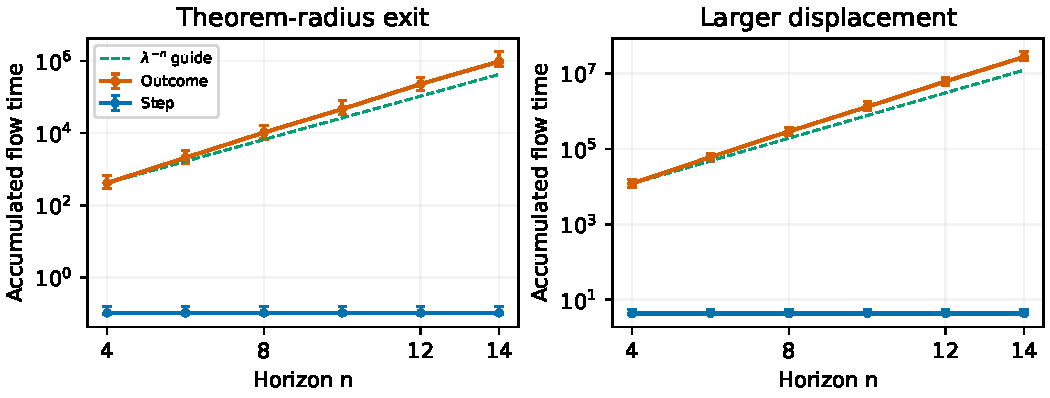
\includegraphics[width=\linewidth]{figures/controlled.pdf}
\caption{\textbf{Outcome displacement times grow with horizon.} Stored runs, seeds $0,1,2$; medians and full seed ranges. Left: exit from $r_0\varepsilon$; right: displacement $0.1\varepsilon\|\tilde\theta\|$, beyond the theorem ball. Dashed guides are $\lambda^{-n}$ with $\lambda=1/2$, anchored at $n=4$. Step exit mainly learns the prior.}\label{fig:controlled}
\end{figure}
Actual transition learning is tested separately by finite-step routing runs. With query--key matrices, relative bias and readout trained from fan-in random weights, step training solves $16/17$ runs within $300$k updates (the remaining run reaches $99.95\%$); outcome solves $0/17$. At $n=6,8,12,16$, step solves $5/5,5/5,4/5,2/2$, with median solve updates $44$k,$61$k,$77$k,$237$k. These runs fix values, embeddings and MLPs but depart from the structured seed and supervise the first state too. Separately, the ten-seed AdamW comparison at $n=16$ reports $95.45\%$ mean step answer accuracy ($93.11\%$ complete-continuation accuracy) and $49.82\%$ outcome answer accuracy. They are empirical evidence outside the theorem, not time-bound verification.

\paragraph{Pretrained Boolean-8.}
Boolean-8 applies eight randomly wired NOT, CNOT, SWAP or Toffoli gates to four bits; there are $16$ answer states. Rank-$8$ LoRA on Qwen2.5-0.5B \citep{qwen2025qwen25,hu2022lora} reaches approximately $98.3\%$ held-out answer accuracy under step supervision and $11.1\%$ under outcome supervision. \Cref{tab:transfer} reports the checked seed summaries, the eightfold outcome budget, and answer-first control. These are synthetic sequential-computation results with a pretrained language model.
\begin{table}[t]
\centering\small
\caption{\textbf{Qwen2.5-0.5B LoRA transfer, with all three seeds.} Held-out greedy answer accuracy (\%). Columns identify seeds $2001,2002,2003$; SD is the sample standard deviation. Boolean-8 has $300$ held-out generated prompts; BBH has $250$ official items per size. The eightfold outcome control uses $6400$ rather than $800$ updates.}
\label{tab:transfer}
\begin{tabular}{@{}lrrrr@{}}
\toprule
Condition & 2001 & 2002 & 2003 & Mean $\pm$ SD\\
\midrule
Boolean-8: step & 95.7 & 99.3 & 100.0 & $98.3\pm2.3$\\
Boolean-8: outcome & 11.3 & 11.0 & 11.0 & $11.1\pm0.2$\\
Boolean-8: answer first & 9.0 & 10.3 & 11.0 & $10.1\pm1.0$\\
Boolean-8: outcome, $8\times$ & 10.7 & 9.0 & 10.3 & $10.0\pm0.9$\\
BBH 3 objects: step & 100.0 & 98.4 & 100.0 & $99.5\pm0.9$\\
BBH 3 objects: outcome & 35.2 & 35.2 & 35.2 & $35.2\pm0.0$\\
BBH 5 objects: step & 100.0 & 100.0 & 46.0 & $82.0\pm31.2$\\
BBH 5 objects: outcome & 94.4 & 83.6 & 80.0 & $86.0\pm7.5$\\
BBH 7 objects: step & 96.4 & 100.0 & 100.0 & $98.8\pm2.1$\\
BBH 7 objects: outcome & 24.4 & 16.0 & 15.2 & $18.5\pm5.1$\\
\bottomrule
\end{tabular}
\end{table}


\paragraph{BIG-Bench Hard object tracking.}
Training examples are generated from benchmark templates using fresh assignments and swaps. Testing uses the official $250$ held-out items at each of three, five and seven objects \citep{suzgun2022challenging}. Traces give every holder's item and its answer-option letter. Step supervision usually helps at three and seven objects. The five-object condition reverses the pattern: outcome achieves $80$--$94\%$, and one step seed reaches only $46\%$. \Cref{tab:transfer} retains all three sizes and all seeds. This reversal limits transfer of the mechanism: counting's contraction coefficient and the theorem's initialization do not characterize pretrained-model optimization on object tracking.

\paragraph{Count-label control.}
A separate ten-seed counting control matches one randomly selected supervised count label per prompt to the outcome count-label budget, with the same formatting labels and $30$k updates. Sparse process training attains mean answer accuracy $97.1,99.8,99.2\%$ for $n=6,8,12$ and solves $27/30$ runs at a $99\%$ threshold; outcome means are $68.5,64.3,51.2\%$, with $0/30$ solved. Matching labels does not match teacher-forced prefix information: sparse process inputs still contain gold running states. The shorter $8$k control was inconclusive and is retained in \cref{app:label-budget}.

\section{Related work}\label{sec:related}
\citet{kim2024parity} prove efficient teacher-forced parity learning with a Transformer and compare learning with and without chain of thought. Their parity setting, prescribed nonlinearity and attention parameterization differ from this paper's biased modular increments, local fixed-ReLU analysis and supplied-routing family. Our contribution is the matched finite-time plateau and persistent transition learning in the specified two-block softmax/ReLU parameterization; it does not subsume parity learning at $p=1/2$.

Makkuva and collaborators analyze Transformer loss landscapes and initialization-dependent dynamics on Markov data \citep{makkuva2025attention,makkuva2024local}. Their Markov next-token setting motivates an architecture-level optimization analysis. Here, the chain is the hidden modular state, and the comparison changes whether its intermediate states are displayed. We use Fourier conditioning rather than identify a separate attracting local minimum.

Gradient barriers based on weak target correlations \citep{shalevshwartz2017failures,abbe2025parities} explain why accessible features can reveal little about a high-order answer. The additional work here is controlling letter support, Taylor remainders and parameter scale in the Transformer, then converting a local loss floor into a trajectory bound. Automata constructions \citep{liu2023automata} show how shallow Transformers can represent sequential shortcuts; they do not imply convergence within the trained subspace. Scratchpad supervision \citep{nye2021scratchpads}, task decomposition \citep{wies2023subtask}, and locality of experience \citep{prystawski2023think} provide related perspectives on intermediate states. Expressivity and statistical advantages of chain of thought \citep{merrill2024expressive,wen2024sparse} concern complementary questions.

\section{Limitations and conclusion}\label{sec:conclusion}
The result concerns population gradient flow, sufficiently small structured initialization, fixed feature maps, aligned tied query--key scalars and supplied routing. It does not establish unrestricted positive training from random initialization. The broader outcome plateau relies on a fixed local ReLU pattern and lasts for a specified initial interval; it is not permanent failure. The constructive executors establish architecture-level expressivity, while leaving capacity and reachability within the trained subspace unresolved. The first transition and free-running error propagation are outside the principal learning guarantee.

A source refinement permits bounded fixed off-direction query--key perturbations only in the binary aligned case, with key orthogonality and relative operator norms at most $1/8$; it does not cover arbitrary weight perturbations. We record its exact scope in \cref{app:robustness} without using it to broaden Theorem~\ref{thm:matched}. Empirical counting and pretrained-model runs change initialization, optimizer or architecture, and the five-object reversal prevents a universal transfer claim. Within the specified regime, however, the same trainable Transformer learns the recurring transition in polynomial time under displayed-state supervision while final-answer supervision remains near chance in expected correct-answer probability for an exponentially long initial interval.
